\section{Assignment 5}

\subsection{3D analysis pipeline}

Using 3D geometry, interesting information can be reconstructed from point clouds. This can be done in combination with the 2D analysis with morphological operators.

\subsubsection{Example 1}

\begin{figure}[h]
\centering
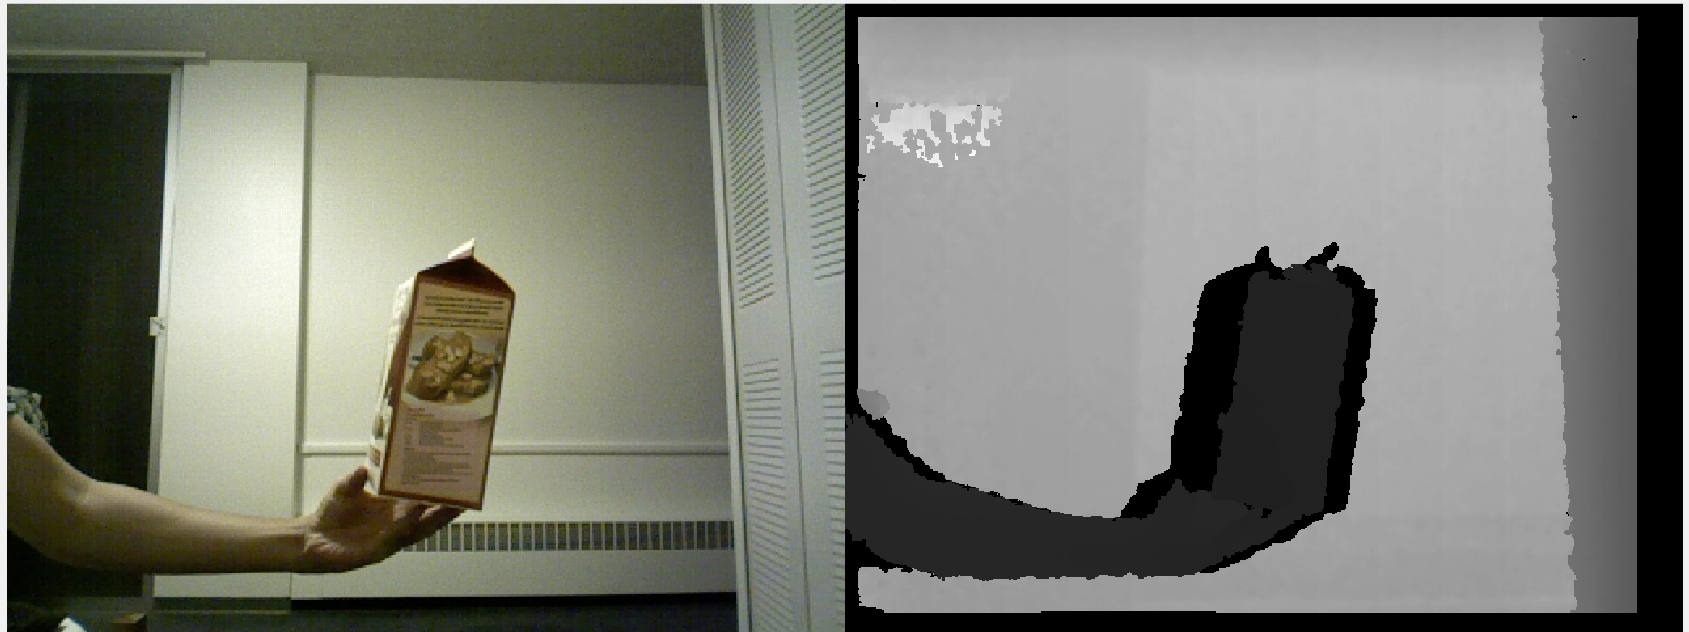
\includegraphics[keepaspectratio,width=0.7\textwidth]{5_box}
\caption{Rgb image (left) vs range image (right)}
\end{figure}
\begin{figure}[h]
\centering
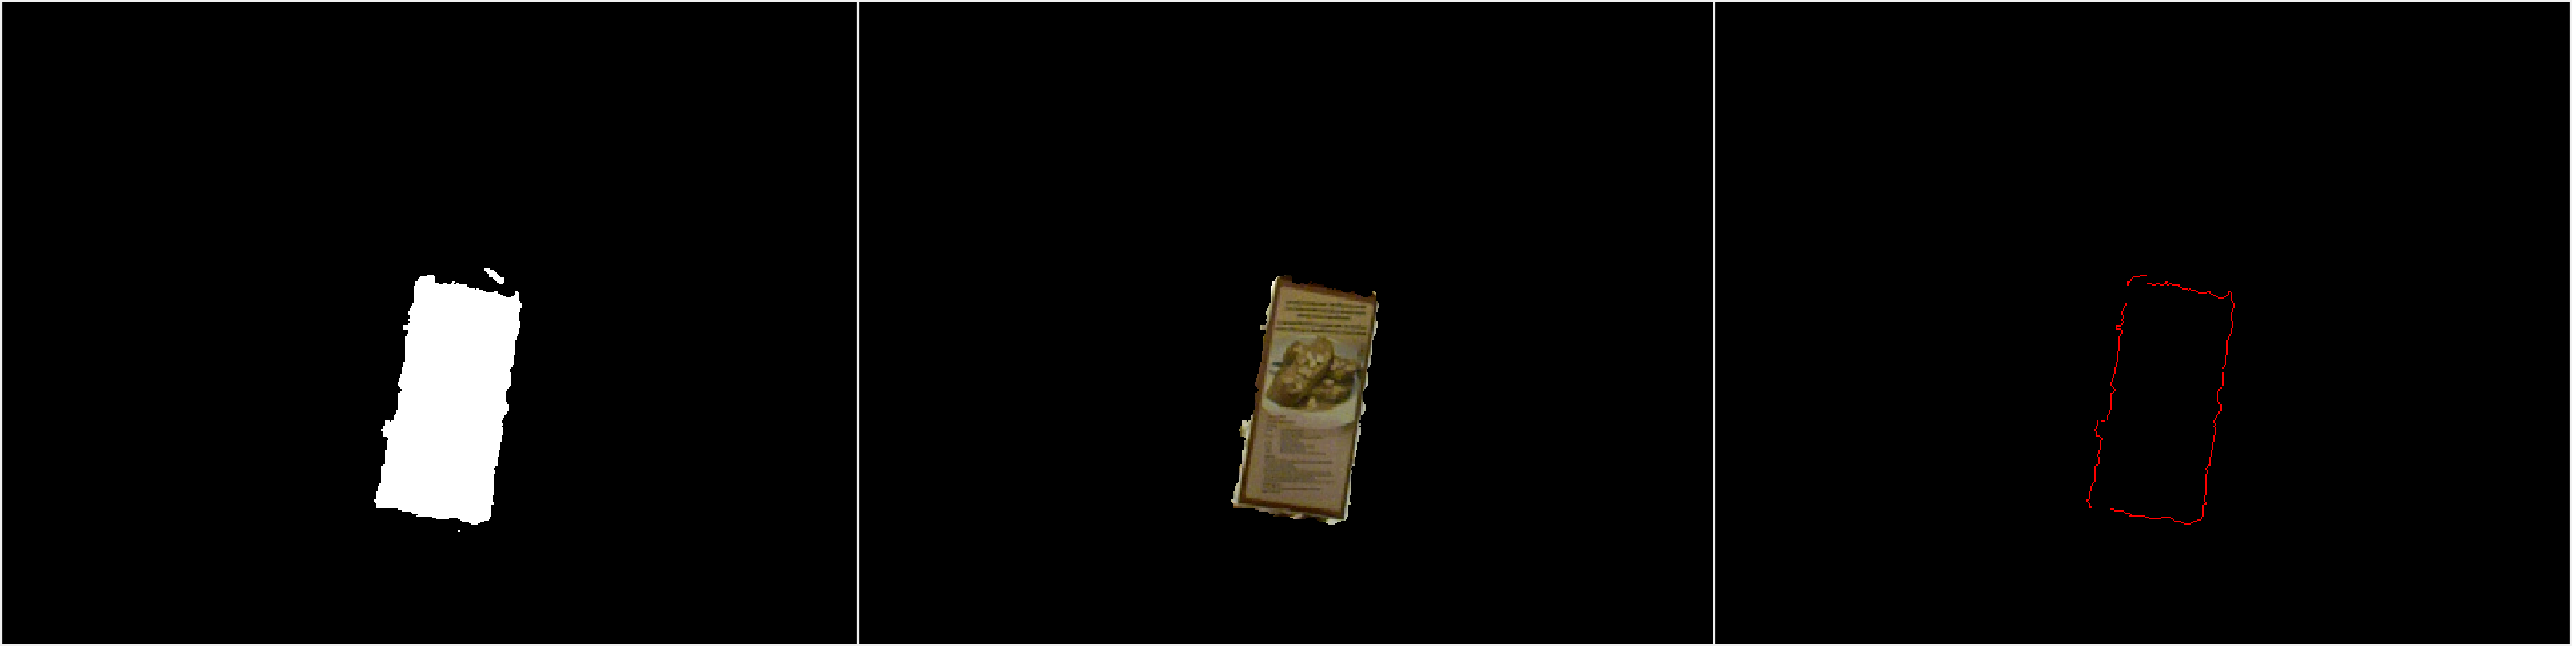
\includegraphics[keepaspectratio,width=0.9\textwidth]{5_box_2d}
\caption{Extracted shapes (left) vs masked image (middle) vs extracted boundary (right)}
\end{figure}
\begin{figure}[H]
\centering
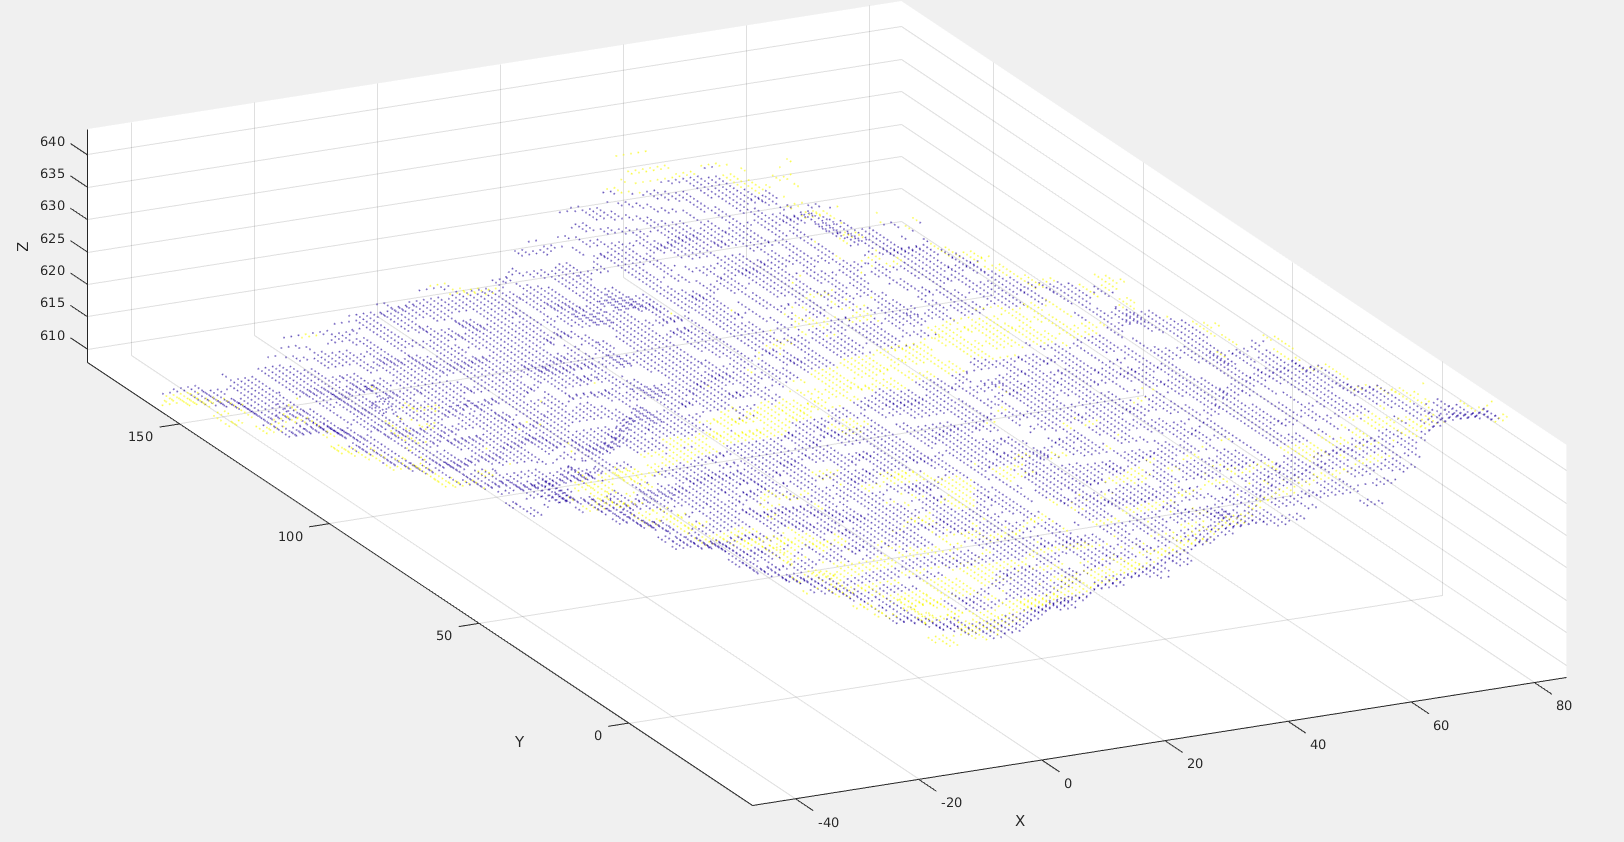
\includegraphics[keepaspectratio,width=0.8\textwidth]{5_box_3d}
\caption{Extracted point cloud}
\end{figure}

\newpage

\begin{figure}[H]
\centering
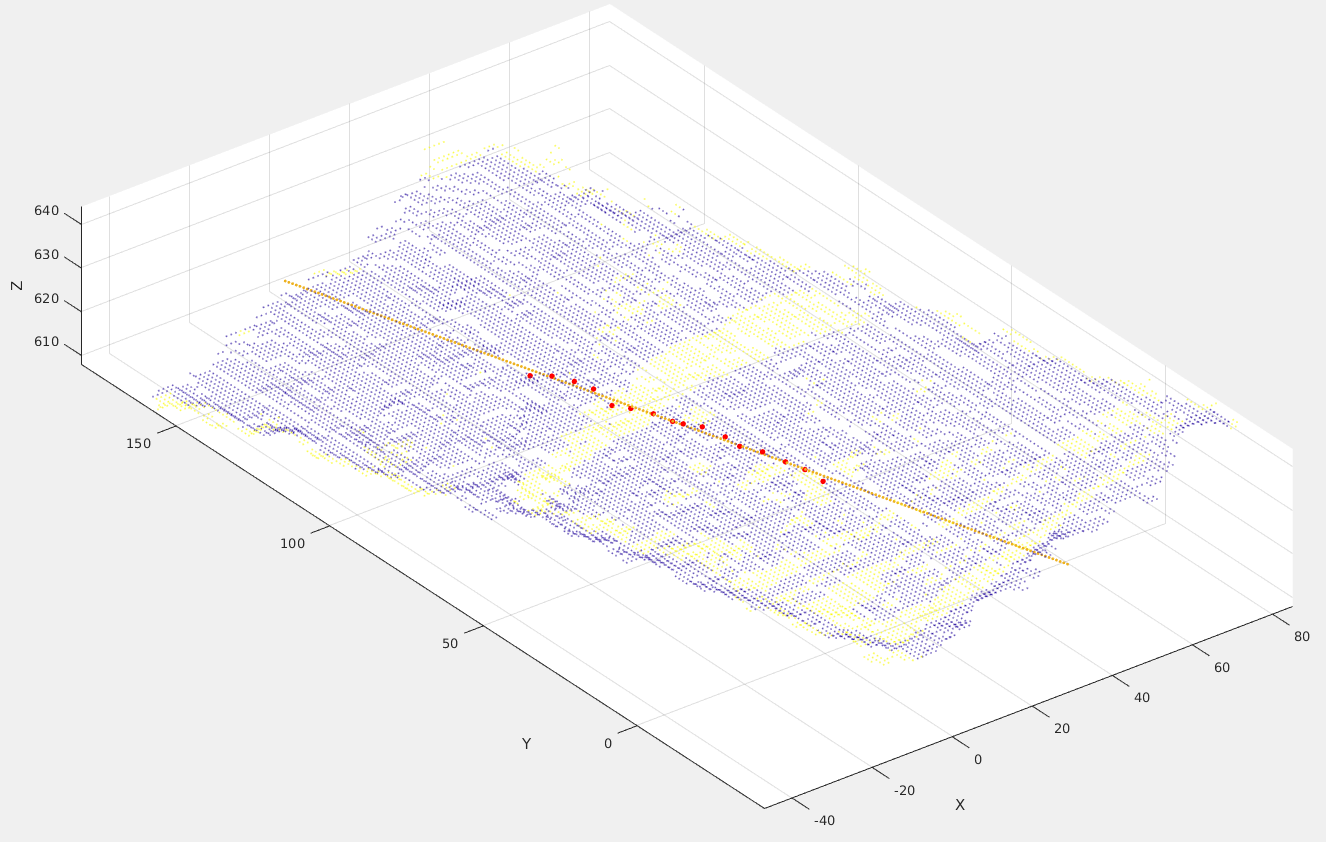
\includegraphics[keepaspectratio,width=0.9\textwidth]{5_box_3d_main}
\caption{Main orientation - 3D line fitting}
\end{figure}
\begin{figure}[H]
\centering
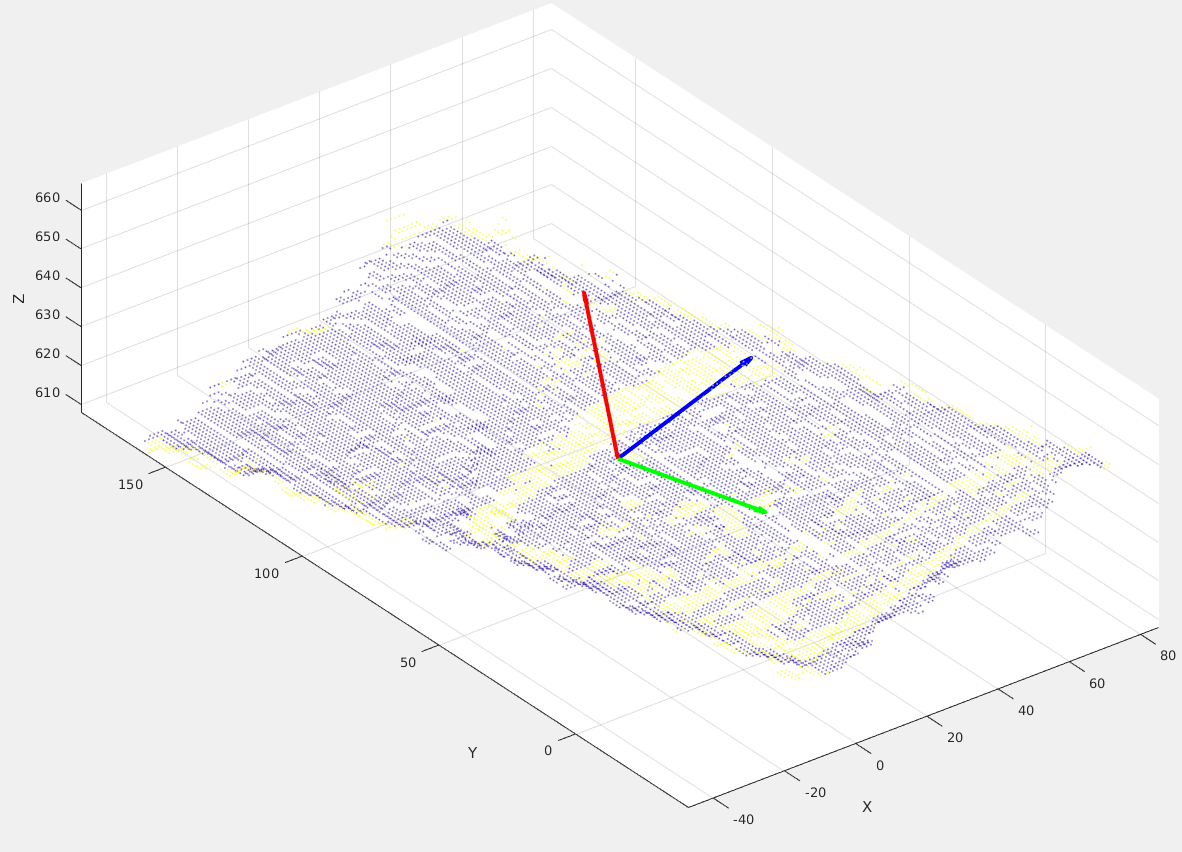
\includegraphics[keepaspectratio,width=0.9\textwidth]{5_box_3d_ori}
\caption{Orientation - PCA}
\end{figure}

\newpage

\begin{figure}[H]
\centering
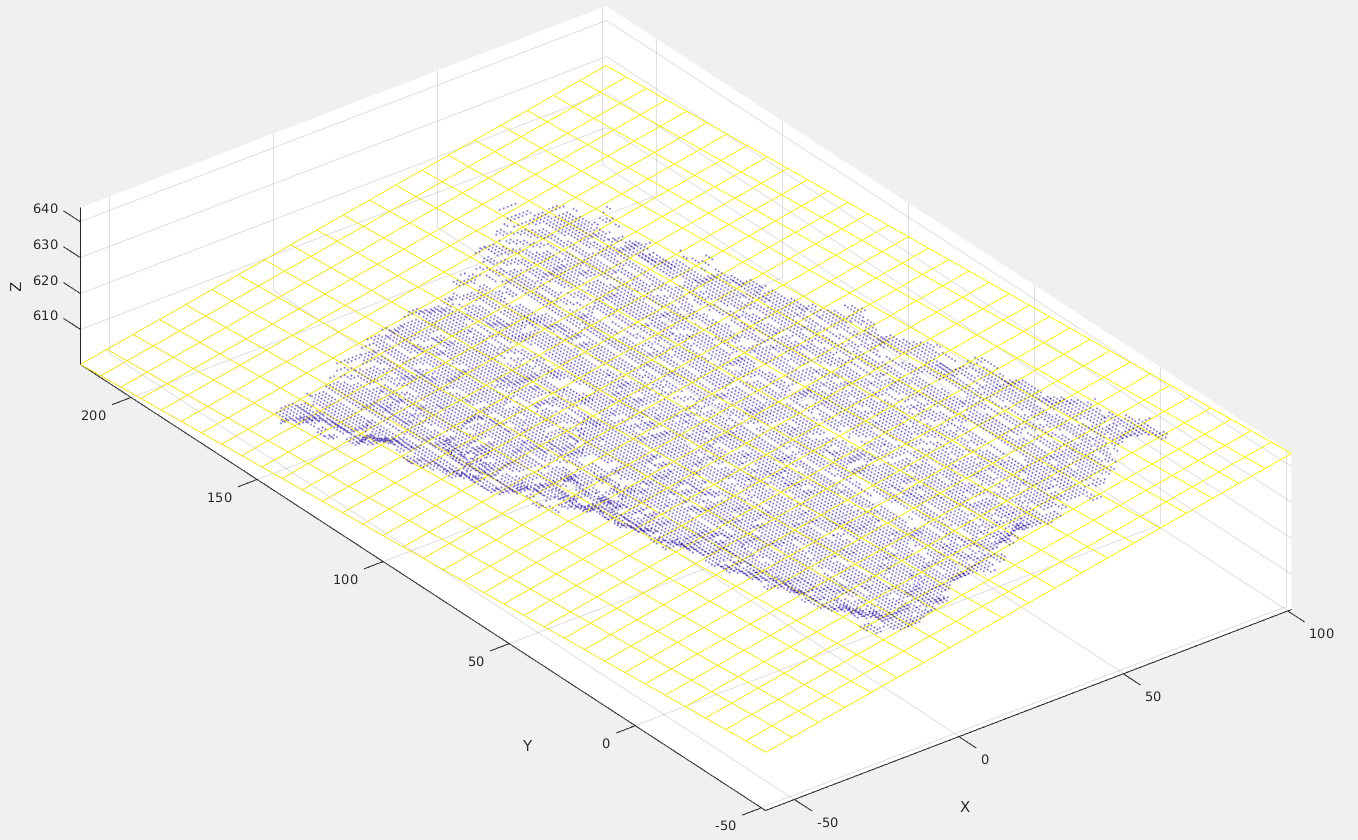
\includegraphics[keepaspectratio,width=0.9\textwidth]{5_box_3d_plane}
\caption{Plane fitting}
\end{figure}
\begin{figure}[H]
\centering
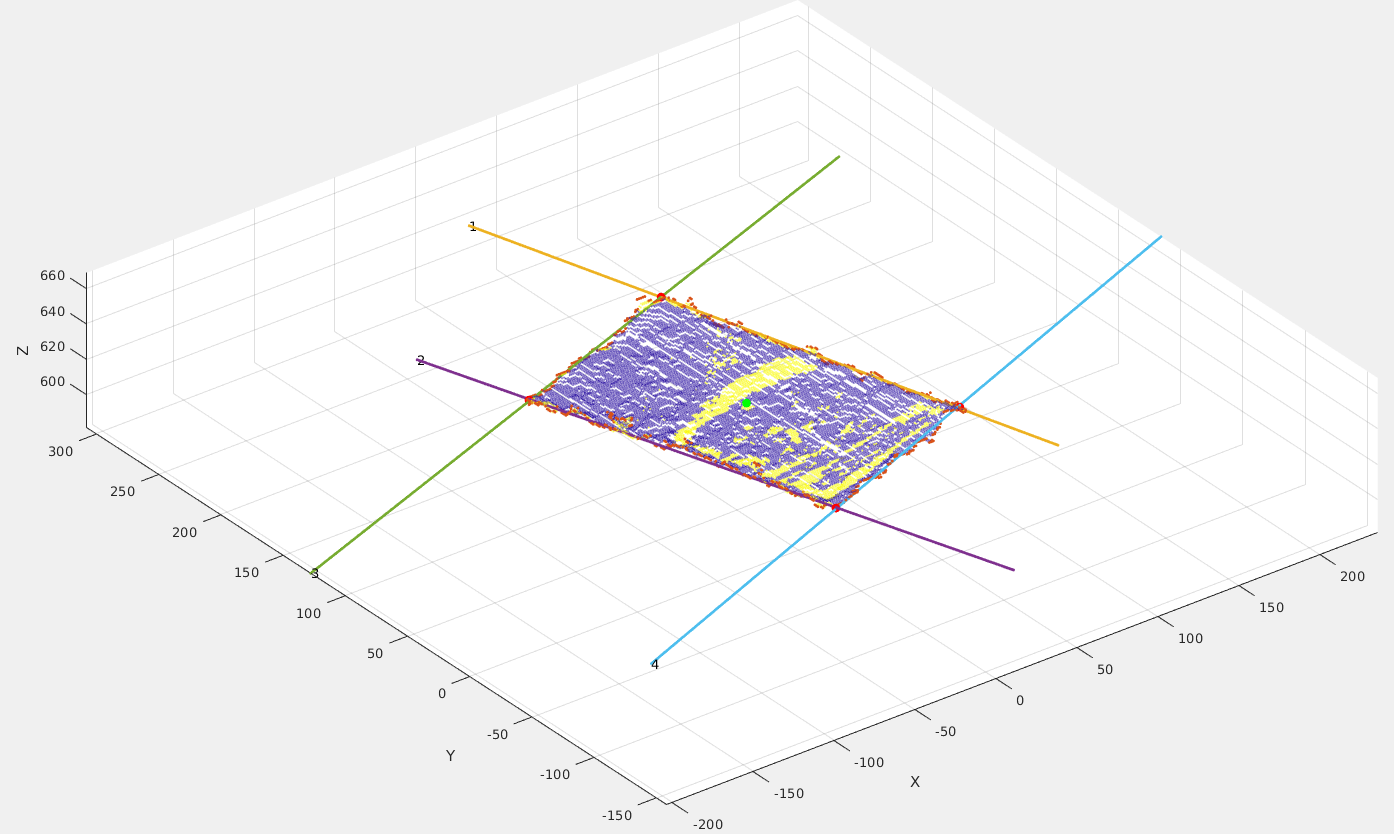
\includegraphics[keepaspectratio,width=0.9\textwidth]{5_box_3d_bound}
\caption{Boundary with 3D line fitting and corner detection}
\end{figure}

\newpage

\subsubsection{Example 2}

\begin{figure}[h]
\centering
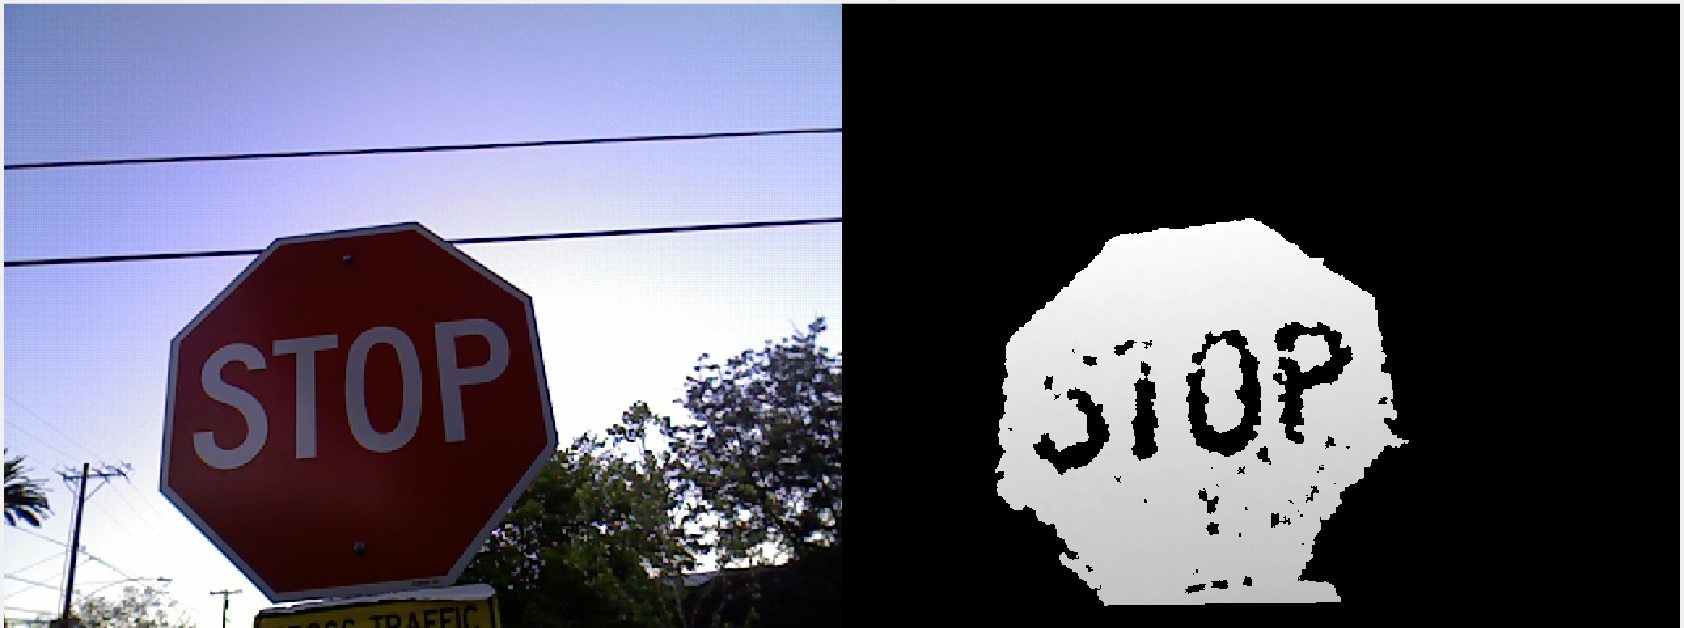
\includegraphics[keepaspectratio,width=0.7\textwidth]{5_stop}
\caption{Rgb image (left) vs range image (right)}
\end{figure}
\begin{figure}[h]
\centering
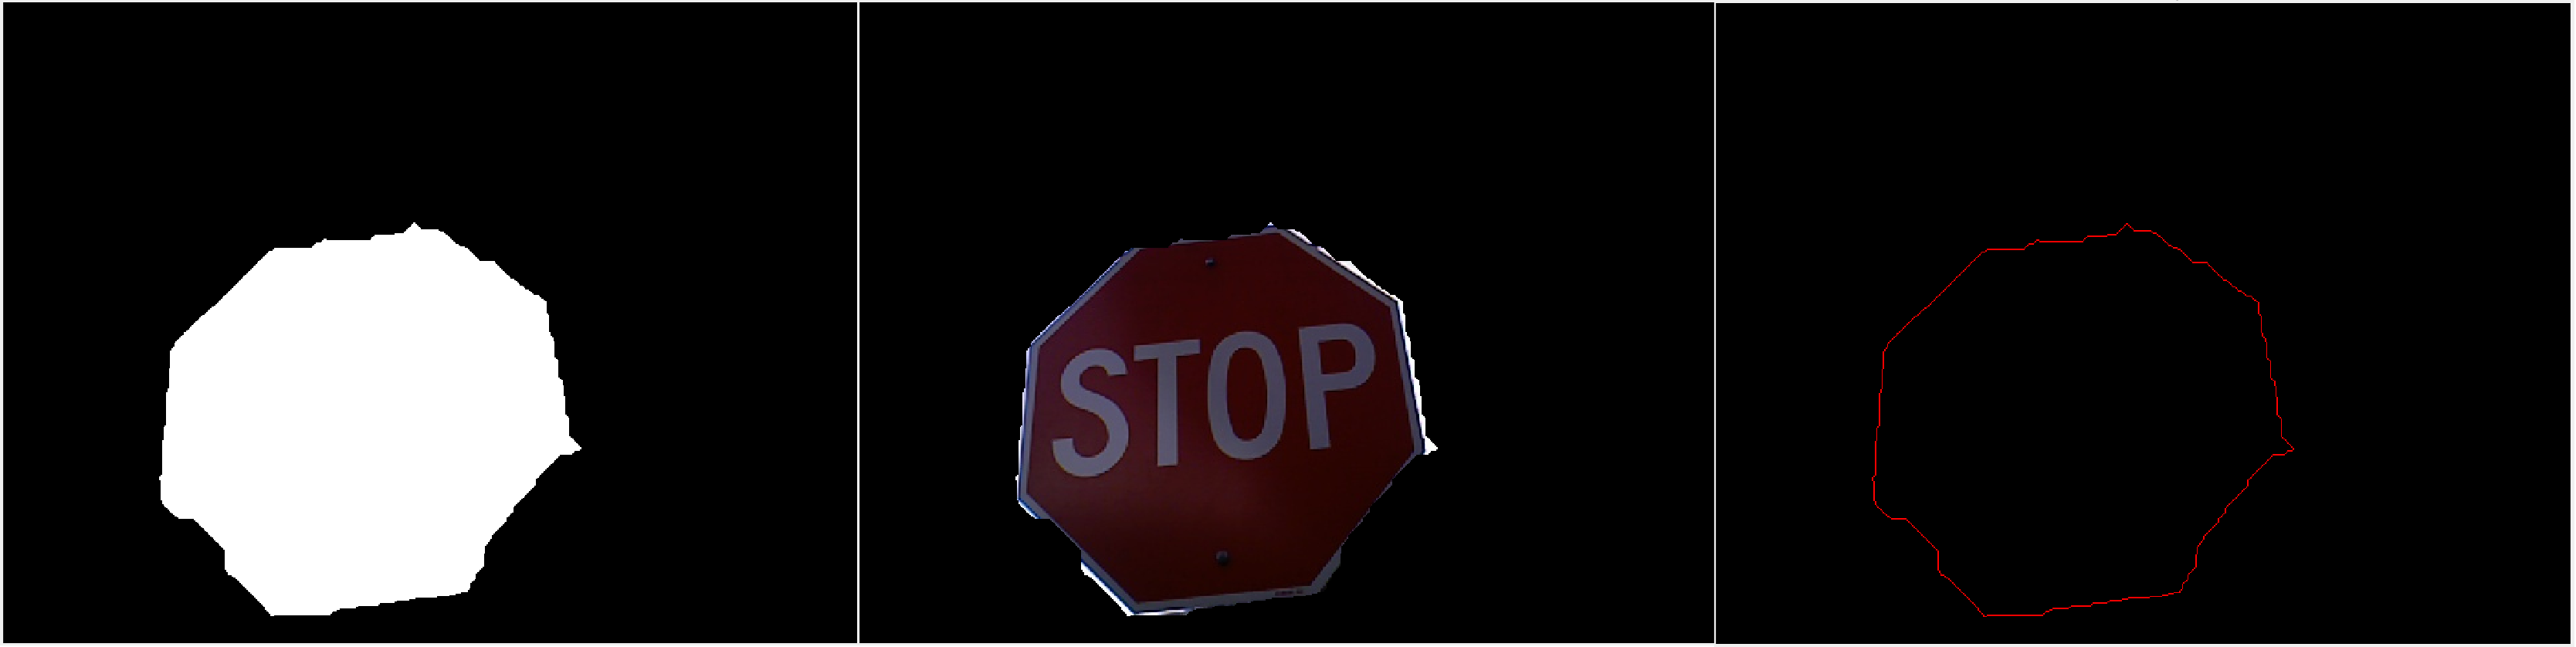
\includegraphics[keepaspectratio,width=0.9\textwidth]{5_stop_2d}
\caption{Extracted shapes (left) vs masked image (middle) vs extracted boundary (right)}
\end{figure}
\begin{figure}[H]
\centering
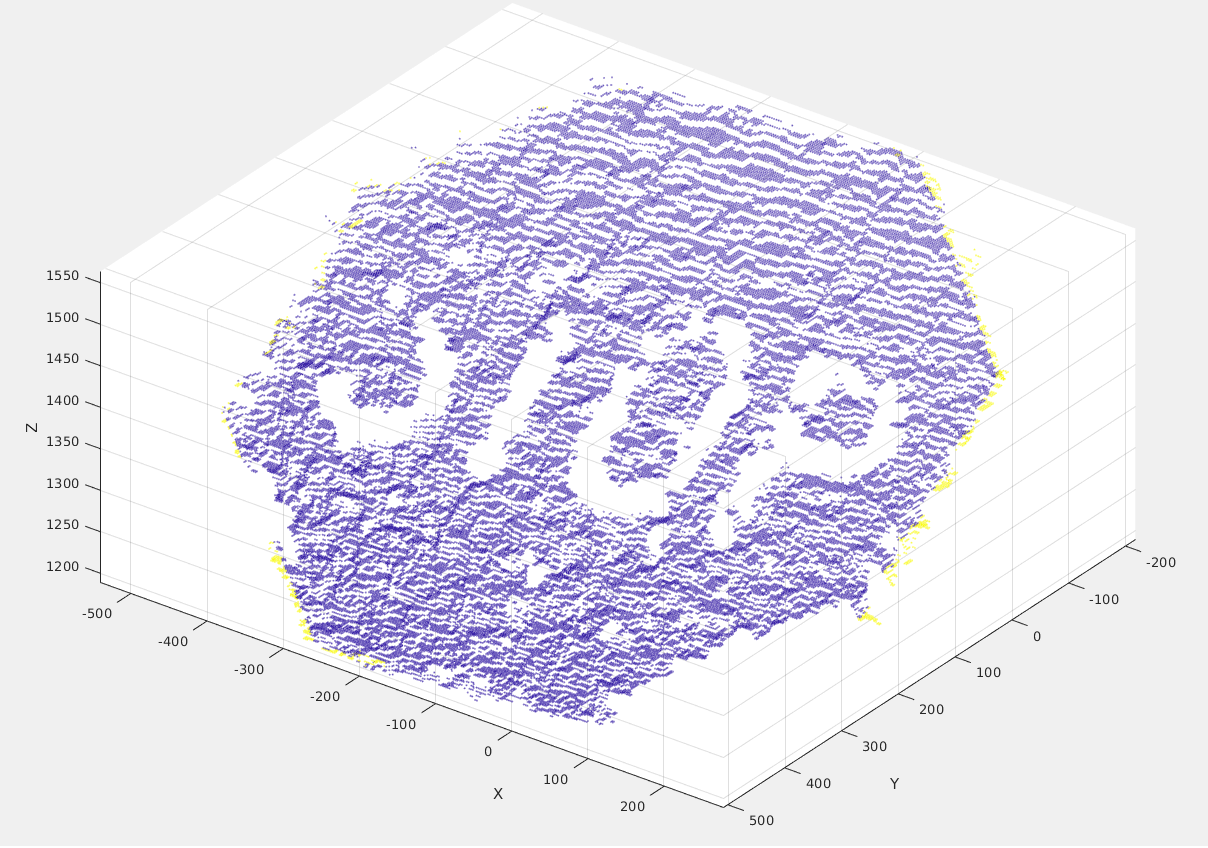
\includegraphics[keepaspectratio,width=0.8\textwidth]{5_stop_3d}
\caption{Extracted point cloud}
\end{figure}

\newpage

\begin{figure}[H]
\centering
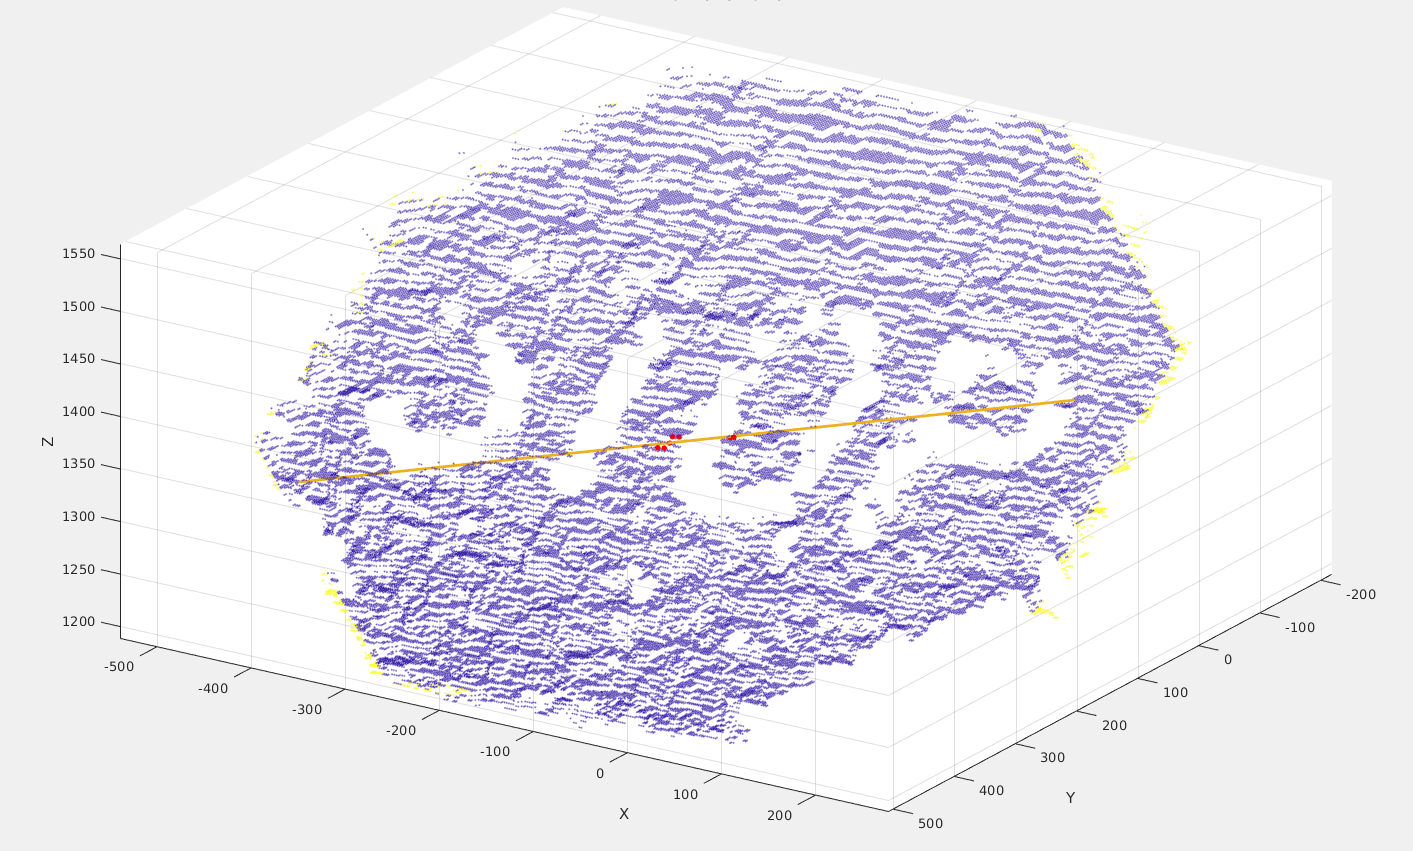
\includegraphics[keepaspectratio,width=0.9\textwidth]{5_stop_3d_main}
\caption{Main orientation - 3D line fitting}
\end{figure}
\begin{figure}[H]
\centering
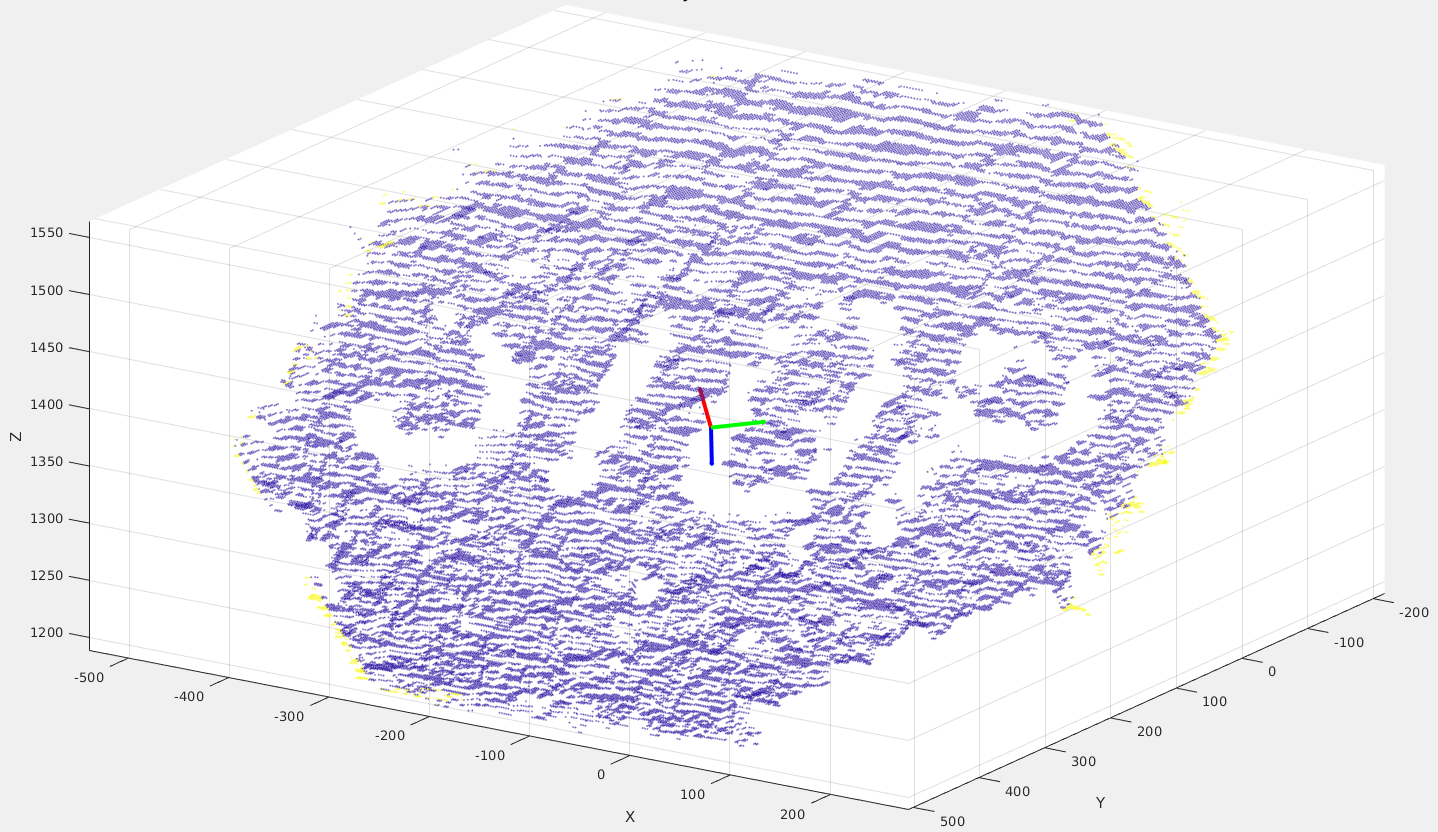
\includegraphics[keepaspectratio,width=0.9\textwidth]{5_stop_3d_ori}
\caption{Orientation - PCA}
\end{figure}

\newpage

\begin{figure}[H]
\centering
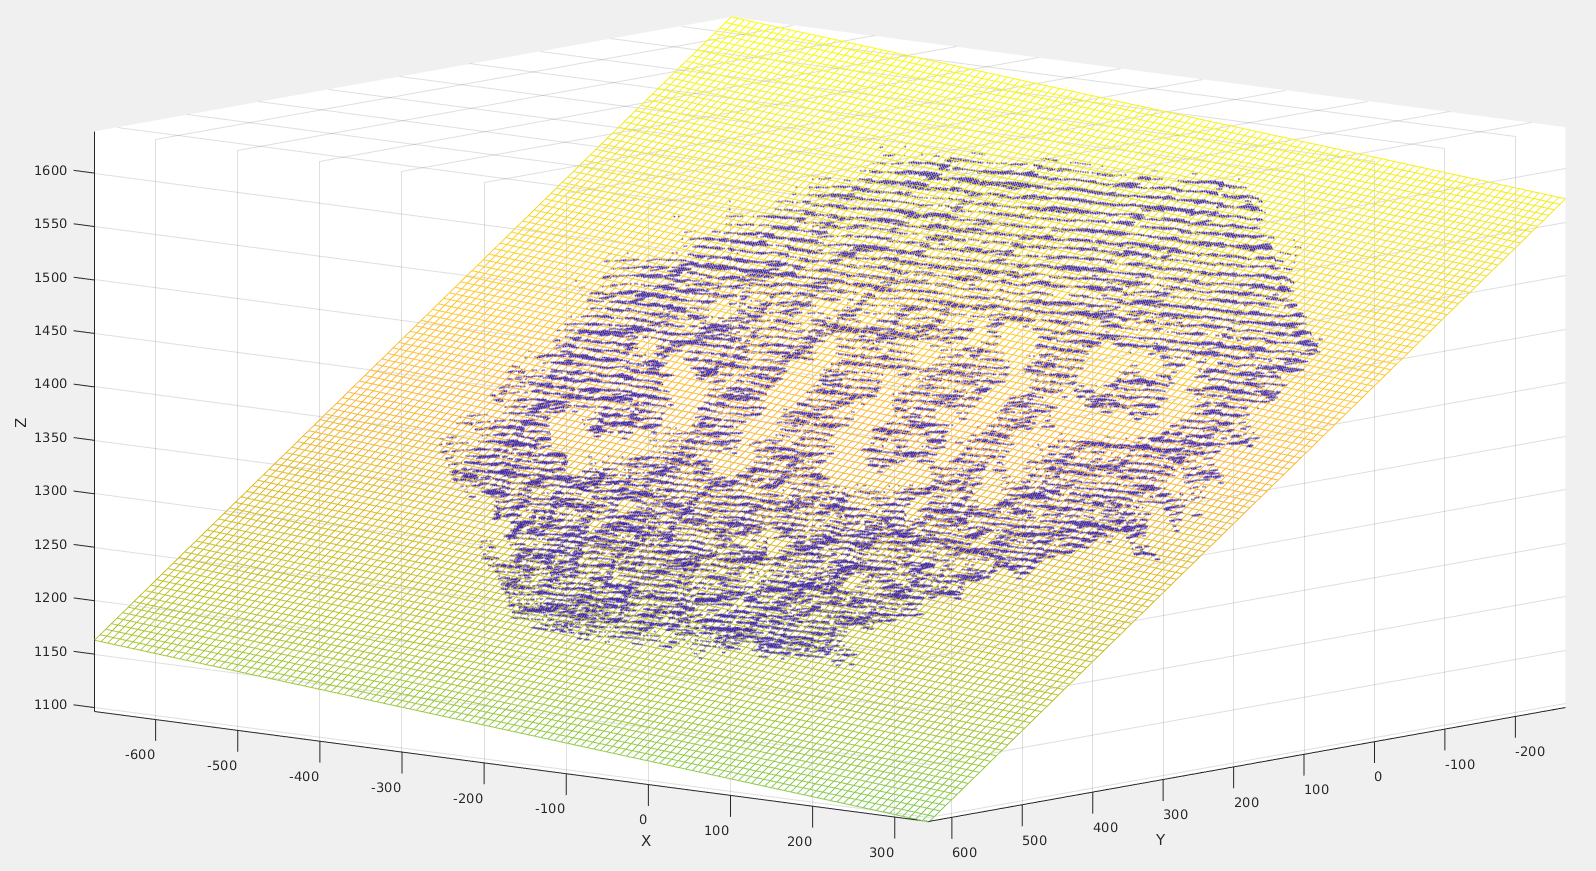
\includegraphics[keepaspectratio,width=0.9\textwidth]{5_stop_3d_plane}
\caption{Plane fitting}
\end{figure}
\begin{figure}[H]
\centering
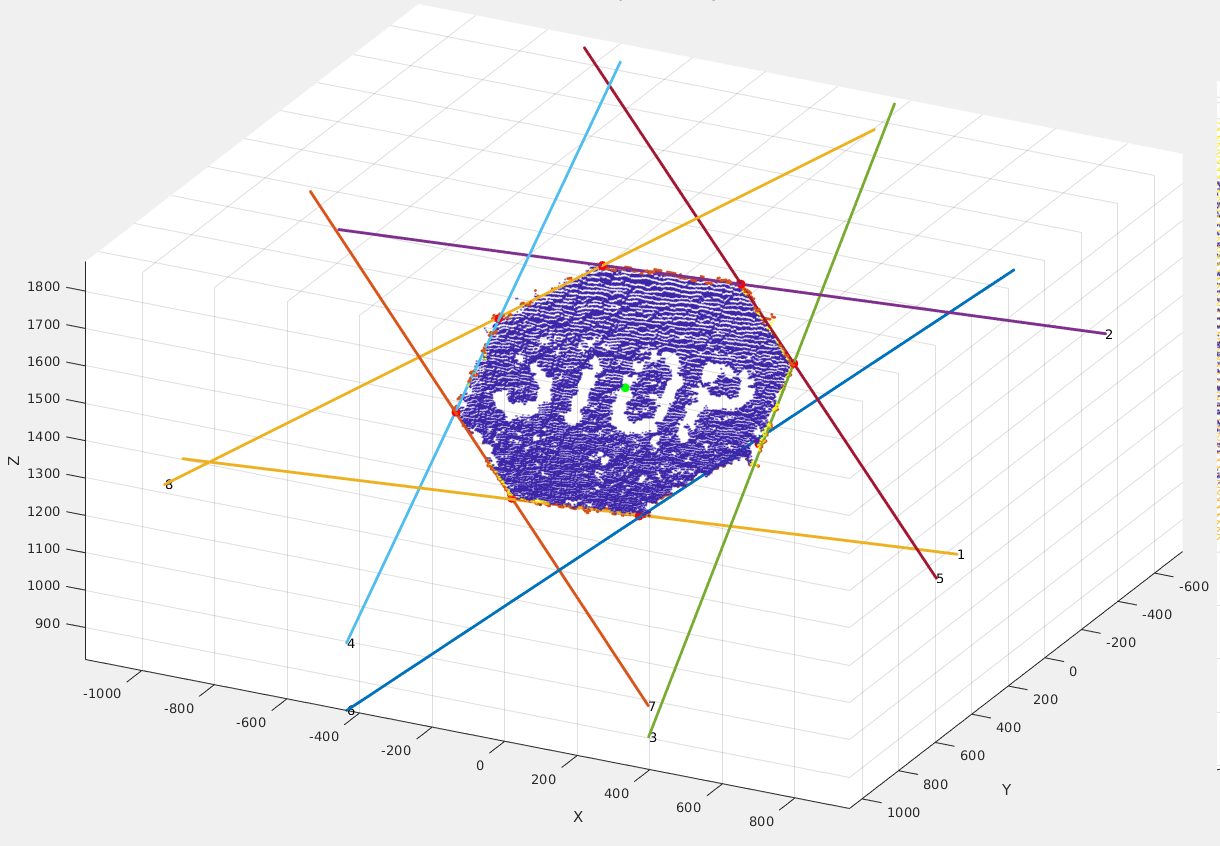
\includegraphics[keepaspectratio,width=0.9\textwidth]{5_stop_3d_bound}
\caption{Boundary with 3D line fitting and corner detection}
\end{figure}

